% Created by tikzDevice version 0.12 on 2019-04-30 14:04:11
% !TEX encoding = UTF-8 Unicode
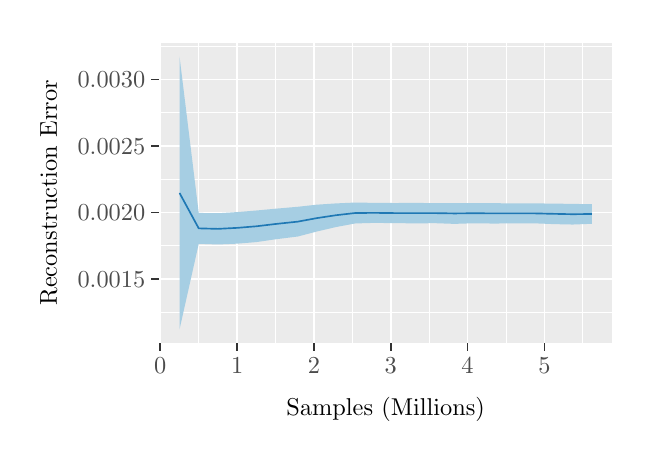
\begin{tikzpicture}[x=1pt,y=1pt]
\definecolor{fillColor}{RGB}{255,255,255}
\path[use as bounding box,fill=fillColor,fill opacity=0.00] (0,0) rectangle (216.81,144.54);
\begin{scope}
\path[clip] (  0.00,  0.00) rectangle (216.81,144.54);
\definecolor{drawColor}{RGB}{255,255,255}
\definecolor{fillColor}{RGB}{255,255,255}

\path[draw=drawColor,line width= 0.6pt,line join=round,line cap=round,fill=fillColor] (  0.00,  0.00) rectangle (216.81,144.54);
\end{scope}
\begin{scope}
\path[clip] ( 47.42, 30.57) rectangle (211.31,139.04);
\definecolor{fillColor}{gray}{0.92}

\path[fill=fillColor] ( 47.42, 30.57) rectangle (211.31,139.04);
\definecolor{drawColor}{RGB}{255,255,255}

\path[draw=drawColor,line width= 0.3pt,line join=round] ( 47.42, 41.80) --
	(211.31, 41.80);

\path[draw=drawColor,line width= 0.3pt,line join=round] ( 47.42, 65.79) --
	(211.31, 65.79);

\path[draw=drawColor,line width= 0.3pt,line join=round] ( 47.42, 89.79) --
	(211.31, 89.79);

\path[draw=drawColor,line width= 0.3pt,line join=round] ( 47.42,113.78) --
	(211.31,113.78);

\path[draw=drawColor,line width= 0.3pt,line join=round] ( 47.42,137.78) --
	(211.31,137.78);

\path[draw=drawColor,line width= 0.3pt,line join=round] ( 61.81, 30.57) --
	( 61.81,139.04);

\path[draw=drawColor,line width= 0.3pt,line join=round] ( 89.57, 30.57) --
	( 89.57,139.04);

\path[draw=drawColor,line width= 0.3pt,line join=round] (117.32, 30.57) --
	(117.32,139.04);

\path[draw=drawColor,line width= 0.3pt,line join=round] (145.08, 30.57) --
	(145.08,139.04);

\path[draw=drawColor,line width= 0.3pt,line join=round] (172.84, 30.57) --
	(172.84,139.04);

\path[draw=drawColor,line width= 0.3pt,line join=round] (200.60, 30.57) --
	(200.60,139.04);

\path[draw=drawColor,line width= 0.6pt,line join=round] ( 47.42, 53.79) --
	(211.31, 53.79);

\path[draw=drawColor,line width= 0.6pt,line join=round] ( 47.42, 77.79) --
	(211.31, 77.79);

\path[draw=drawColor,line width= 0.6pt,line join=round] ( 47.42,101.78) --
	(211.31,101.78);

\path[draw=drawColor,line width= 0.6pt,line join=round] ( 47.42,125.78) --
	(211.31,125.78);

\path[draw=drawColor,line width= 0.6pt,line join=round] ( 47.93, 30.57) --
	( 47.93,139.04);

\path[draw=drawColor,line width= 0.6pt,line join=round] ( 75.69, 30.57) --
	( 75.69,139.04);

\path[draw=drawColor,line width= 0.6pt,line join=round] (103.45, 30.57) --
	(103.45,139.04);

\path[draw=drawColor,line width= 0.6pt,line join=round] (131.20, 30.57) --
	(131.20,139.04);

\path[draw=drawColor,line width= 0.6pt,line join=round] (158.96, 30.57) --
	(158.96,139.04);

\path[draw=drawColor,line width= 0.6pt,line join=round] (186.72, 30.57) --
	(186.72,139.04);
\definecolor{fillColor}{RGB}{166,206,227}

\path[fill=fillColor] ( 54.87,134.11) --
	( 61.81, 77.60) --
	( 68.75, 77.48) --
	( 75.69, 77.90) --
	( 82.63, 78.47) --
	( 89.57, 79.12) --
	( 97.60, 79.82) --
	(104.53, 80.58) --
	(111.47, 81.04) --
	(118.41, 81.35) --
	(125.35, 81.23) --
	(132.29, 81.18) --
	(140.32, 81.20) --
	(147.26, 81.16) --
	(154.20, 81.17) --
	(161.14, 81.10) --
	(168.08, 81.11) --
	(175.01, 81.07) --
	(183.04, 81.03) --
	(189.98, 80.98) --
	(196.92, 80.85) --
	(203.86, 80.77) --
	(203.86, 73.67) --
	(196.92, 73.40) --
	(189.98, 73.56) --
	(183.04, 73.84) --
	(175.01, 73.81) --
	(168.08, 73.76) --
	(161.14, 73.86) --
	(154.20, 73.64) --
	(147.26, 73.89) --
	(140.32, 73.83) --
	(132.29, 73.91) --
	(125.35, 74.00) --
	(118.41, 73.80) --
	(111.47, 72.51) --
	(104.53, 70.89) --
	( 97.60, 69.07) --
	( 89.57, 68.07) --
	( 82.63, 67.06) --
	( 75.69, 66.49) --
	( 68.75, 66.20) --
	( 61.81, 66.45) --
	( 54.87, 35.50) --
	cycle;
\definecolor{drawColor}{RGB}{31,120,180}

\path[draw=drawColor,line width= 0.6pt,line join=round] ( 54.87, 84.81) --
	( 61.81, 72.02) --
	( 68.75, 71.84) --
	( 75.69, 72.20) --
	( 82.63, 72.77) --
	( 89.57, 73.60) --
	( 97.60, 74.45) --
	(104.53, 75.73) --
	(111.47, 76.78) --
	(118.41, 77.57) --
	(125.35, 77.62) --
	(132.29, 77.54) --
	(140.32, 77.51) --
	(147.26, 77.52) --
	(154.20, 77.41) --
	(161.14, 77.48) --
	(168.08, 77.43) --
	(175.01, 77.44) --
	(183.04, 77.43) --
	(189.98, 77.27) --
	(196.92, 77.13) --
	(203.86, 77.22);
\end{scope}
\begin{scope}
\path[clip] (  0.00,  0.00) rectangle (216.81,144.54);
\definecolor{drawColor}{gray}{0.30}

\node[text=drawColor,anchor=base east,inner sep=0pt, outer sep=0pt, scale=  0.88] at ( 42.47, 50.76) {0.0015};

\node[text=drawColor,anchor=base east,inner sep=0pt, outer sep=0pt, scale=  0.88] at ( 42.47, 74.76) {0.0020};

\node[text=drawColor,anchor=base east,inner sep=0pt, outer sep=0pt, scale=  0.88] at ( 42.47, 98.75) {0.0025};

\node[text=drawColor,anchor=base east,inner sep=0pt, outer sep=0pt, scale=  0.88] at ( 42.47,122.75) {0.0030};
\end{scope}
\begin{scope}
\path[clip] (  0.00,  0.00) rectangle (216.81,144.54);
\definecolor{drawColor}{gray}{0.20}

\path[draw=drawColor,line width= 0.6pt,line join=round] ( 44.67, 53.79) --
	( 47.42, 53.79);

\path[draw=drawColor,line width= 0.6pt,line join=round] ( 44.67, 77.79) --
	( 47.42, 77.79);

\path[draw=drawColor,line width= 0.6pt,line join=round] ( 44.67,101.78) --
	( 47.42,101.78);

\path[draw=drawColor,line width= 0.6pt,line join=round] ( 44.67,125.78) --
	( 47.42,125.78);
\end{scope}
\begin{scope}
\path[clip] (  0.00,  0.00) rectangle (216.81,144.54);
\definecolor{drawColor}{gray}{0.20}

\path[draw=drawColor,line width= 0.6pt,line join=round] ( 47.93, 27.82) --
	( 47.93, 30.57);

\path[draw=drawColor,line width= 0.6pt,line join=round] ( 75.69, 27.82) --
	( 75.69, 30.57);

\path[draw=drawColor,line width= 0.6pt,line join=round] (103.45, 27.82) --
	(103.45, 30.57);

\path[draw=drawColor,line width= 0.6pt,line join=round] (131.20, 27.82) --
	(131.20, 30.57);

\path[draw=drawColor,line width= 0.6pt,line join=round] (158.96, 27.82) --
	(158.96, 30.57);

\path[draw=drawColor,line width= 0.6pt,line join=round] (186.72, 27.82) --
	(186.72, 30.57);
\end{scope}
\begin{scope}
\path[clip] (  0.00,  0.00) rectangle (216.81,144.54);
\definecolor{drawColor}{gray}{0.30}

\node[text=drawColor,anchor=base,inner sep=0pt, outer sep=0pt, scale=  0.88] at ( 47.93, 19.56) {0};

\node[text=drawColor,anchor=base,inner sep=0pt, outer sep=0pt, scale=  0.88] at ( 75.69, 19.56) {1};

\node[text=drawColor,anchor=base,inner sep=0pt, outer sep=0pt, scale=  0.88] at (103.45, 19.56) {2};

\node[text=drawColor,anchor=base,inner sep=0pt, outer sep=0pt, scale=  0.88] at (131.20, 19.56) {3};

\node[text=drawColor,anchor=base,inner sep=0pt, outer sep=0pt, scale=  0.88] at (158.96, 19.56) {4};

\node[text=drawColor,anchor=base,inner sep=0pt, outer sep=0pt, scale=  0.88] at (186.72, 19.56) {5};
\end{scope}
\begin{scope}
\path[clip] (  0.00,  0.00) rectangle (216.81,144.54);
\definecolor{drawColor}{RGB}{0,0,0}

\node[text=drawColor,anchor=base,inner sep=0pt, outer sep=0pt, scale=  0.88] at (129.37,  4.25) {Samples (Millions)};
\end{scope}
\begin{scope}
\path[clip] (  0.00,  0.00) rectangle (216.81,144.54);
\definecolor{drawColor}{RGB}{0,0,0}

\node[text=drawColor,rotate= 90.00,anchor=base,inner sep=0pt, outer sep=0pt, scale=  0.88] at ( 10.59, 84.81) {Reconstruction Error};
\end{scope}
\end{tikzpicture}
